% !TEX root = NSF_SuperCDMS_SNOLAB_OPS.tex

\subsection{Calibration of Si and Ge \scs Detectors (\WBS 1.1)}
\MP{
\begin{itemize}
	\item rename to measure the nuclear recoil ionization yield at very low energies
    \item I think we should add a section on testing the electronic recoil calibration signal using LEDs
    \item we need to write this section with the understanding that 0V operation has a natural nuclear recoil ionization scale.
\end{itemize}
}

\label{sec:calibration}

A major focus of the SuperCDMS pre-operations program is to measure the nuclear recoil energy response in both Ge and Si down to 100 eV and eventually down to $\sim$30\eV.  This will match the energy thresholds we expect to achieve with the initial experiment and with upgraded detector towers.  These measurements are crucial for optimizing the operational parameters of, as well as achieving science in the next three years with the first production HV SuperTower at the Cryogenic Underground TEst (\cute) facility in \SNOLAB. Thus it is important to perform these measurements as early as possible, ideally completing them before data taking with the HV tower at \cute begins.

The signature of a WIMP-like dark matter interaction is a spectrum of low-energy nuclear recoils. \MP{WIMP DM is excluded < 10GeV ... we are looking largely for assymmetric dark matter models} The nuclear recoils produce both ionization and phonons.  The ionization yield (also know as quenching factor), which is the fraction of recoil energy that goes into the ionization, is recoil energy dependent.  A calibration of the nuclear recoil energy scale requires a measurement of the ionization yield, both its mean and its distribution, for all recoil energies of interest.

% The signature of a WIMP-like dark matter interaction is a spectrum of low-energy nuclear recoils. The observed signal in the HV detectors is a linear combination of the primary phonon and ionization signals, and is dominated by the ionization which is amplified by the Neganov-Luke effect.  This observed energy is converted to nuclear recoil energy based on understanding of the detector ionization yield (also know as quenching factor), which is the fraction of recoil energy that goes into the ionization channel.  A calibration of the nuclear recoil energy scale is hence effectively a measurement of the ionization yield. -- old text, Alan, 02/11/2016

\begin{figure}
\centering
\includegraphics[width=0.75\textwidth, trim={0 0 0 20}, clip]{Figures/Yield_Baseline_vs_Literature_SiGe}
\caption{Comparison of a simulation of the proposed ionization yield measurement compared with existing measurements of the mean ionization yield from the literature. The proposed measurement, shown following a Lindhart ionization yield model, has the potential to provide essential data on the ionization yield mean and statistical fluctuations for dark matter rate calculations in the lowest energy ranges. 
The colored scatter points correspond to the simulated ionization yield as a function of recoil energy, superimposed on the \(\pm1\sigma\) statistical uncertainty band from Eq.~\ref{eq:yielderr} (note that the blue \(\pm1\sigma\) bands only account for the statistical uncertainty due to phonon energy resolution and neutron scattering angle, whereas the actual points also include the effect of electron-hole production statistics, i.e., the Fano Factor). The gray diamonds indicate the mean value of the calculated yield from the simulation, and the vertical bars are the square root of the variance. Figure adapted from~\cite{2013APh....48....8B,1965PhRv..138.1815S,1990PhRvD..42.3211G}.
%\vspace{-3ex}
}
\label{fig:exp_vs_litt}
\end{figure}
Figure~\ref{fig:exp_vs_litt} shows current mean ionization yield measurements in germanium and silicon detectors made with a variety of detector technologies, along with the theoretical prediction from the Lindhard model~\cite{1964PhL....12..126L}. Also shown (and discussed fully in the subsequent sections) are a set of simulated yield measurements %done by the \UF group
demonstrating what would be possible with the proposed work, superimposed on the current state of knowledge of the low energy nuclear recoil yield in germanium~\cite{2013APh....48....8B} and silicon~\cite{1965PhRv..138.1815S,1990PhRvD..42.3211G,1992PhRvA..45.2104D,Chavarria:2016arXiv}. Highlighting the importance of experimental data, a recent measurement, made by the DAMIC collaboration (top panel of Figure~\ref{fig:exp_vs_litt}), indicates that the ionization yield in Si is significantly different from the theoretical predictions of Lindhard at and below 1\keV.  Projecting the deviations down to 100\eV suggests even larger discrepancies.

For SuperCDMS, the interplay of ionization yield, trigger threshold and experimental sensitivity is complex.  As the ionization signal is detected via its conversion to phonons by the Luke-Neganov effect, the total phonon signal measured includes both primary phonons from the recoil and Luke-Neganov phonons from primary ionization. In Figure~\ref{fig:SensitivityYVScanHV}, calculations for Si show how the sensitivity can vary with different ionization yield assumptions.  Furthermore, systematic bias from uncertainty in the ionization yield can be reduced and sensitivity to the lowest masses regained by operating at reduced voltage at the cost of higher background in the signal region (as demonstrated by the extreme case of 0\,V, which is used here to show the theoretical maximum effect).  Both issues demonstrate the need to measure the ionization yield of \scdmssnolab HV detectors by the time science runs at \cute begin.
\begin{figure}[htp]
\centering
\includegraphics[width=0.48\textwidth]{Figures/Sensitivity_Si_YV_Scan}
\includegraphics[width=0.48\textwidth]{Figures/Sensitivity_Ge_YV_Scan}
\caption{Left panel: Sensitivity scan of SuperCDMS SNOLAB Si HV detectors for different yield and analysis thresholds. Black is the nominal projected sensitivity, which uses the DAMIC yield function~\cite{Chavarria:2016arXiv} and extrapolates the yield curve down to 40\,eV~\cite{SuperCDMSSensitvitiy:2016arXiv}. Grey is Lindhard theory for comparison. Orange is the sensitivity projection for operation of the detector with zero voltage across the crystal. The red line shows the sensitivity from an analysis that sets the threshold at the lowest recoil energy for which data on ionization yield exists (675\,eV). The region to the left of the red line highlights the WIMP parameter space that requires new experimental data for ionization-measuring detectors. Right panel: Same as Left but for Ge HV. The black line uses Lindhard theory, orange is zero-voltage operation, and red applies an analysis threshold of 254\,eV.
%\vspace{-3ex}
}
\label{fig:SensitivityYVScanHV}
\end{figure}

\subsubsection{Measurement Strategy}

We propose to perform a precision measurement of the ionization yield in this energy range first at a neutron beam facility with small prototype detectors and subsequently using a D--D neutron generator with full-sized SuperCDMS SNOLAB detectors.  In both these setups, the energy of the incoming neutron is known and the deposited nuclear recoil energy in the detector is determined kinematically by measuring the outgoing neutron angle. By directly measuring the ionization signal in the target/detector it is then possible to perform a direct measurement of the ionization yield. 

%%%%%%%%%%\subsubsection{The Voltage-Assisted Calorimetric Ionization Detection Technique}
\SuperCDMS detectors determine the properties of a particle interaction by measuring the energy deposited in two different physical channels: the phonon and ionization channels. When an interaction takes place in the detector the total recoil energy of an interaction is initially divided among a population of prompt athermal phonons and a population of charged excitations (\textit{i.e.}, electrons and holes). A uniform electric field of a few V/\(\!cm\) causes the electrons and holes to drift to opposite surfaces where they are detected with a capacitively-coupled charge amplifier. The motion of the charged excitations in the crystal under the influence of the applied electric field creates a population of phonons known as Luke-Neganov phonons. These release to the phonon system an amount of energy equal to the work required to drift the charges through the field across the resistive crystal, i.e., $E_{Luke} = n_{eh}\,e\,V$, where $n_{eh}$ is the number of electron hole pairs made in the recoil, and $e\,V$ is the electron charge times the voltage across the crystal.  The total phonon energy $E_{ph}$ measured in the detector for a given recoil energy $E_r$ is,
\begin{equation}
\label{eq:yield}
E_{ph} = Er + E_{Luke} = E_r \left ( 1+\frac{e\,V\,Y}{\mathcal{E}_{eh}} \right )
\end{equation}
where $\mathcal{E}_{eh}$ is the average electron equivalent energy required to form an electron hole pair, $Y$ is the ionization yield

Effective ionization resolutions on the order of few eV (corresponding to individual e-h pairs) can be achieved using the technique of voltage-assisted calorimetric ionization detection which was first used by the \SuperCDMS experiment in a low-mass WIMP search using the current iZIP detectors~\cite{2014PhRvL.112d1302A,Agnese:2015nto}. By applying a high voltage (HV) across the crystal the ionization signal can be effectively amplified and measured using the phonon sensors since the energy released into the Luke-Neganov phonon population will dwarf the intrinsic recoil phonons. The detector is then being effectively operated as a phonon-based charge amplifier in which the gain of the signal is proportional to the applied voltage, and the readout channel has a fixed resolution.  The measurement uncertainty of the ionization yield, measured using Eq.~\ref{eq:yield} , the measured total phonon energy and an independent determination of the recoil energy (\textit{e.g}., from a neutron scattering angle measurement), is: 
\begin{equation}
\sigma_y= \frac{\mathcal{E}_{eh}}{e\,V}\frac{\sqrt{E_{rec}^2\sigma_{ph}^2+E_{ph}^2\sigma_{rec}^2}}{E_{rec}^2}
\label{eq:yielderr}
\end{equation}
Since the ionization yield uncertainty depends both on the phonon channel resolution and the bias voltage, a worse than expected phonon resolution can be compensated for with a higher voltage bias. %Above a bias of 500\volt , however, the uncertainty becomes dominated by the uncertainty in the recoil energy (from the event kinematics measurement), taken to be 100\eV in this calculation.

Figure~\ref{fig:exp_vs_litt} shows the result of a simulation % by the \UF group, 
with neutrons incident on a test detector with 50\eV resolution, superimposed on the current state of knowledge of the low energy nuclear recoil yield in germanium~\cite{2013APh....48....8B} and silicon~\cite{1965PhRv..138.1815S,1990PhRvD..42.3211G,1992PhRvA..45.2104D,Chavarria:2016arXiv}. This simulation shows that this experiment will have the ability to reliably identify the mean value of the ionization yield down to \(\sim 50\eV\). The horizontal spread in each population of events arises from a given neutron detector accepting a \(\pm 1\deg\) range of scattering angles.

At the improved, but still conservative, energy resolution of 10\eV (this value is twice the expected 5\eV resolution of the \SuperCDMS R\&D devices that will be used for the measurement) it becomes possible to identify the number of electron-hole pairs produced by a given recoil as shown in Figure~\ref{fig:eh_counting}. This will provide an important piece of information regarding the statistical nature of ionization production and allow us to perform a direct measurement of the Fano factor down to the lowest recoil energies.

\MP{include quantization plot from Stanford.  Switch plots to show quantized sensitivities}

\begin{figure}[t]
\centering
\includegraphics[width=\textwidth]{Figures/Phtot-Hist-Neutron-beam-HiRes-G4}
\caption{
Demonstration of the ability to identify the number of discrete electron-hole pairs (indicated by the dashed vertical lines) created by a low energy nuclear recoil. The combination of high bias voltage and excellent energy resolution allows for the measurement of the Fano factor even with limited statistics.
%The figure is based on simulations performed by the \UF group.
%\vspace{-2ex}
}
\label{fig:eh_counting}
\end{figure}

\subsubsection{Yield Calibration with a Neutron Beam at TUNL (\WBS 1.1.1)}
\label{sec:tunl}

The Triangle Universities Nuclear Lab (\tunl) data taking campaign will occur in the first year of this grant (see schedule in Figure~\ref{fig:ops-schedule}). \tunl operates a facility capable of delivering a mono-energetic neutron beam with energies in the range of 30\keV to a few\MeV~\cite{TUNL:website,Theprecisionquench:2014tw}. A tandem Van de Graaff is used to accelerate protons and collide them with a \isotope[7]{Li} target. The resulting \isotope[7]{Li}(p,n)\isotope[7]{Be} reaction produces a neutron that is primarily collinear with the proton beam. At a proton threshold energy of 1.88\MeV the reaction produces neutrons with 29.7\keV kinetic energy which are kinematically constrained to be in the forward direction. Increasing the proton energy allows for the production of neutrons with a range of kinetic energies and directions, however by selecting a particular direction (e.g. collinear with the proton beam) a unique neutron energy is obtained~\cite{1999NIMPB.152....1L}.

The neutron beam passes through a 2 foot high-density polyethylene (HDPE) block which collimates the beam and absorbs unwanted reaction products (such a \(\gamma\)-rays) and is directed to the target location. Backing detectors  (5cm inch diameter plastic scintillator, with sensitivity to neutrons down to 6\keV) surround the interaction site and detect the scattered neutron providing knowledge of the scattering angle and timing of the event, and can be positioned around the interaction point as needed. The TUNL facility currently has 32 such detectors and is in the process of deploying 200 more to provide a solid angular coverage of almost \(1\pi\) steradian. The additional neutron detectors are expected to become available in January of 2017. One of the most useful features of the facility is its ability of providing a pulsed beam, which in conjunction with the backing detectors' timing resolution of \(< 4\,\)ns allows for an excellent rejection of events due to pileup, multiple scatter or radioactive backgrounds, and also provides a secondary measure of the neutron energy through its time-of-flight.

The details of the backing detector configuration will be investigated and optimized in the early stages of the proposed work plan in order to obtain an experimental setup that allows for making the measurement at the the desired level of accuracy in a minimum amount of beam time.

%%%%%%%%%%\subsubsection{Calibration at a Neutron Beam Facility}
%Calibration at a neutron beam facility, such as TUNL~\cite{TUNL:website}, is attractive because the beam energy can be tuned as low as $\sim$30\keV and an extensive secondary neutron detector array is available for use~\cite{Theprecisionquench:2014tw}. 
The Northwestern \SuperCDMS group owns an Adiabatic Demagnetization Refrigerator (ADR) that can be transported to TUNL to perform such a measurement.  The ADR can cool small, special-purpose Ge and Si HV detectors, each with mass of a few grams. Detectors of this size are produced as part of the \SuperCDMS R\&D program and are available for these measurements. Two such detectors (one made of Si, one of Ge) will be installed in the ADR so the \tunl measurements can be done without warming up or opening the cryostat.

The kinematics at a neutron beam result in an excellent recoil energy resolution: for a \(1\deg\) uncertainty in the direction of the scattered neutron, the reconstructed energy resolution is on the order of 4\eV for a 100\eV recoil. This value is close the the expected 5\eV resolution of the \SuperCDMS phonon sensors, and as seen in equation~\ref{eq:yielderr}, is optimal for achieving excellent ionization yield resolution. The neutron beam measurements will be used to obtain the highest resolution ionization yield measurements at the lowest energies allowing us to study in detail the physics and statistics of electron-hole pair production via nuclear recoils at their creation threshold.


\subsubsection{The TUNL Experimental Campaign}

The simulation in Figure~\ref{fig:exp_vs_litt} assumed \(10^3\) events for each recoil energy. We investigated a feasable set of operational parameters necessary for obtaining such statistics in the actual data while minimizing the amount of multiple scatter, pileup and background events in the data. The two driving variables are the detector response time, and the interaction probability of a neutron with the detector. 

Based on a conservative detector recovery time of \(\tau=1ms\) we wish to keep the interaction rate in the detector below 100~Hz to minimize pulse pileup. The mean free path of 30\keV neutrons in silicon (germanium) is \(\sim 2cm\) (\(\sim 2.3cm\)), which gives a 18\% (16\%) probability for a single neutron to interact in the 4mm thick test detector. This can lead to a large number of simultaneous interactions in the detector from a single beam pulse contaminating the data. This effect can be mitigated by decreasing the average number of neutrons per beam bunch. A mean number of neutrons per bunch of \(n_{mean}=0.4\) results in less than 3\% contamination from simultaneous interactions. The combination of \(n_{mean}=0.4\) and a bunch frequency of \(\frac{1}{600\mu s}\) results in a net detector interaction rate of 100~Hz. Such an operating mode is well within the capabilities of the facility and given the $< 4$~ns timing resolution of the backing detectors there will be no difficulties distinguishing which beam bunch produced a particular interaction~\cite{barbeau:2014}. Assuming that each backing detector covers an angle of \(\left( 1\deg\right)^2\), that they are positioned in groups of 10 at each of 20 angles, and that the net neutron interaction rate in the detector is 100~Hz, we can estimate the total active beam time required to obtain the necessary statistics to be around 12 hours. The data for the different recoil energies is collected simultaneously by the grid of \(>200\) backing detectors at 20 specific scattering angles. Assuming a net efficiency of five to six hours of beam time per calendar day, it is reasonable to expect that a data acquisition period of a few days is sufficient for a particular measurement. Data will be taken for both a prototype Si and Ge detector, at multiple bias voltages and operating conditions (such as crystal temperature) during a three week running window. An additional week before and after the data acquisition campaign for assembly/disassembly and verifying the operation of the detector at the TUNL facility will also be required.

\subsubsection{Data Contamination}
\begin{figure}[tb]
\centering
\includegraphics[width=0.45\hsize]{Figures/single_multiple_scatters_geant}
\includegraphics[width=0.45\hsize]{Figures/Delta_t_histograms}
\caption{Left panel: %Distribution of 
Energy deposited in the detector as a function of neutron scattering angle. The orange band band represents events in which the neutron scattered only once within the detector without interacting with the surrounding material. Events which multiply scatter within the detector are shown in blue, and events which interact with the Al or Cu surrounding the detector are shown in green and red respectively. Right panel: Histogram of the event delay times, i.e. the time between the arrival of a beam bunch and the detection of a neutron in the backing detectors. The delay was defined such that \(\Delta t=0\) for a non-scattered neutron, and the backing detectors' timing resolution is \(< 4\,\)ns.
\vspace{-3ex}
}
\label{fig:geant}
\end{figure}

Environmental radiation background and neutron interactions with the material surrounding the detectors have the potential to contaminate the data. A proper understanding of these interactions requires a detailed Monte-Carlo simulation. The results from a basic \geant simulation done by our U. Florida collaborators and shown in Figure~\ref{fig:geant} are still quite informative. They simulated the interactions of a neutron beam with a detector surrounded by a 1mm thick copper housing, contained in a 1cm thick aluminum cylindrical shell (which represents the cryostats vacuum jacket). The figure's left panel shows the distribution of energy deposited in the detector as a function of neutron scattering angle. The thick orange band represents events in which the neutron scattered only once within the detector without interacting with the surrounding material.  Multiple scatters within a detector, as well as events in which the neutron interacts with the surrounding material are also shown. The right panel shows the delay time distribution (the time between the arrival of a beam bunch and the detection of a neutron in the backing detectors). It can be seen that a time based acceptance cut can remove a large portion of multiply scattered events and interactions in the surrounding material. It is worth noting however, that even without applying any selection criteria, the simulation shows that contamination from such events is less than 5\% for all recoil energies \(< 1\keV\).



\subsubsection{D-D Generator Measurements at NEXUS (\WBS 1.1.2)}
\label{sec:ddcal}

\MP{What about testing the concept of measuring nuclear recoil ionization yields with Cf by measuring 0V, 50V, 100V. This would give us the possibility of using Cf for insitu calibration of all detectors in SNOLAB (or at NEXUS) extremely easily}

There are several challenges associated with calibrating large cryogenic solid-state detectors in a fixed neutron beam.  These massive detectors require a dilution refrigerator to operate at millikelvin temperatures, and such refrigerators are not portable.  Adiabatic Demagnetization Refrigerators, although portable, lack the cooling capacity to effectively operate these detectors. Furthermore, underground calibrations are critical for large cryogenic detectors. When operated on the surface, the time between events from cosmic radiation can be less than the recovery time required for the phonon sensors to return to equilibrium. \MP{this just isn't true. We have a compton background of 40Hz (25ms) and a falltime which is <100us ... we have 250 falltimes on average between comptons. The bigger problem is muons [perhaps what you were referring to] ... muons occur @1Hz and have a 200ms thermal falltime.  We find that with a muon cut with 50\% passage, we get rid of this to the point that it's subdominant to other noise sources ... it's definitely a penalty (50\% livetime) ... but it's not a true deal breaker ... remember that the livetime of our old DAQ was only 15\%. We still take more good data now with the muon cut then we ever took with the old DAQ at UCB)}.

The portability of a D--D generator allows for neutron calibration at underground locations, such as \nexus, described in Section~\ref{sec:nexus}. 

%MOVED to NEXUS section
%\begin{figure}[t]
%\centering
%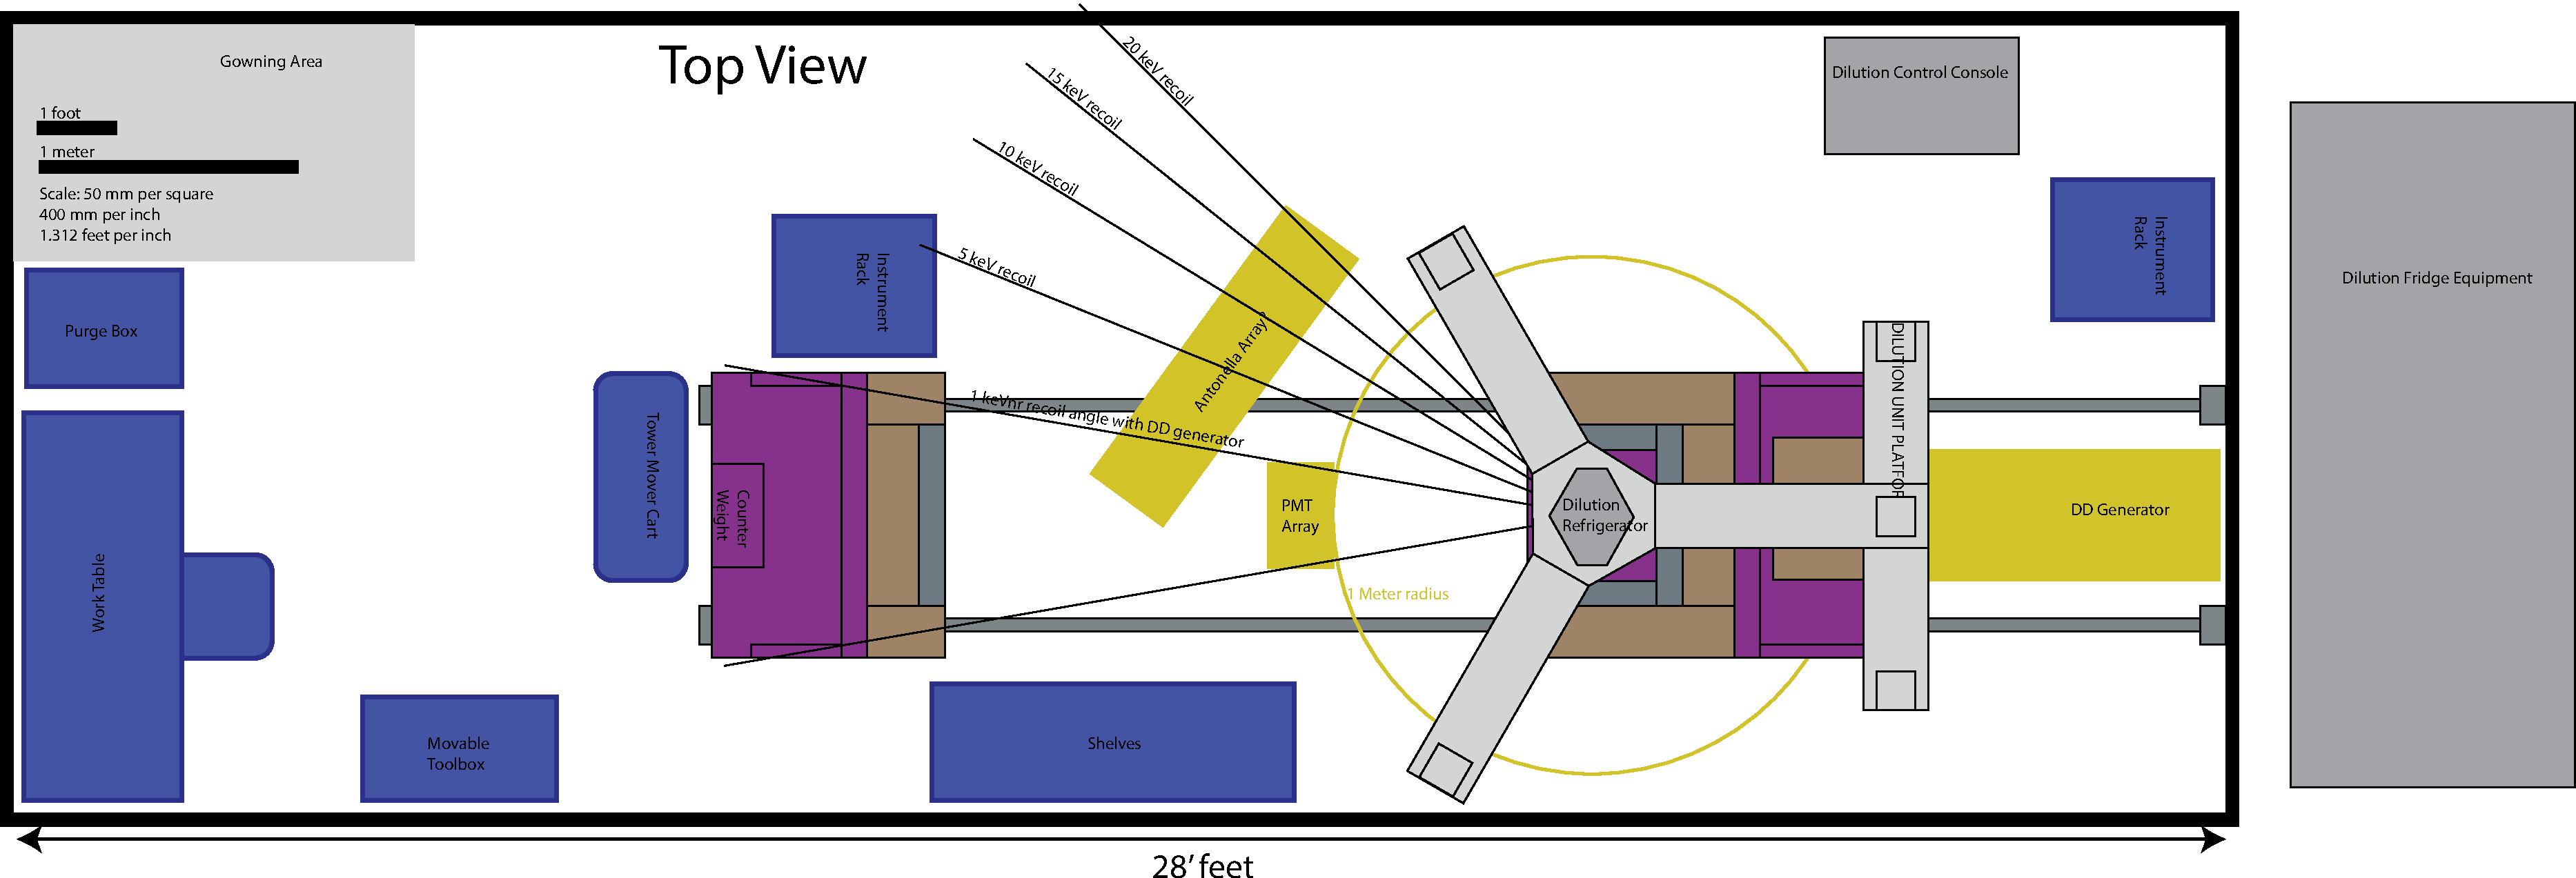
\includegraphics[width=\textwidth]{Figures/NEXUS-Layout-YieldMeas}
%\caption{\nexus layout schematic. The outer box delineates the clean room to be placed 100 m underground in the \numi access tunnel. The blue boxes are support equipment, while the grey, brown, and purple structures are the passive shield, which is on rollers and half of it is moved out to the left to allow the neutron backing detectors to be placed. The D--D generator is shown as a yellow box on the right, with neutrons passing through a collimating hole in the shield toward the detectors. Neutrons hit the HV detectors in the dilution refrigerator and scatter into angles as labeled depending on the recoil energy. An existing array from Fermilab will cover the wider angles between up to 20~keV, while a purpose-made fine-grain neutron detector PMT array will cover the recoil energies below 1~keV.\vspace{-2ex}}
%\label{fig:nexus}
%\end{figure}


Calibration with a D-D generator requires borated poly shielding to collimate the D-D neutrons into a beam and a moderate amount of lead shielding to block the capture gammas. Additionally, secondary neutron detectors are needed to measure the scattered neutrons at a given angle.  The ANTONELLA collaboration has a neutron detector array, that was created exactly for this purpose and is currently available for use.  This array covers relatively large angles of scatter ($>$10$^\circ$).  With this array, we can measure nuclear recoils down to a few keV with the D-D beam energies.  Measurement down to 100 eV requires fabrication of a finer-grained neutron array. Design of such an array, with the reuse of 1.3 cm Hamamatsu photomultiplier tubes salvaged from the SELEX experiment, will be pursued by the U. Florida and Fermilab groups. The setup is schematically shown in Figure~\ref{fig:nexus}.

\MP{Has this array been procured?  If not then you are just doing nuclear recoil ionization yield measurements @ a few keV}

In \SuperCDMS detectors, there are energy-scale effects that are degenerate with measurement of the ionization yield and can vary with detector parameters such as the strength of the electric field, fabrication of the phonon sensors, and even the impurity levels in a given crystal.  To understand these systematic effects, it is important to perform the calibration on detectors that will have the same electric field and style of phonon sensor.  Furthermore, it is highly desirable to perform measurements on several different detectors of the same type, operated at several bias voltages.  \MP{explain} 

The primary challenge of the D--D calibration is the relatively high energy (2.5\MeV) of the neutrons compared to the recoil energies of interest (100\eV). For a \(1\deg\) uncertainty in the direction of the scattered neutron the reconstructed energy resolution of a 100\eV recoil becomes \(\sim 30\eV\). This uncertainty becomes the limiting factor in the measured yield resolution. One way to compensate for this effect is to use a fine-grained neutron array to determine the neutrons' very small scattering angles. An angular resolution of \(\sim0.125\deg\) is needed to achieve the same recoil energy resolution as with the 30\keV\ \tunl neutron beam. The resulting scattering rates per secondary neutron channel will be approximately 60 times lower compared to the rates at a neutron beam facility. The lower detection rates, in turn, lead to longer data acquisition times and an increased sensitivity to environmental backgrounds. Studies will optimize the tradeoff between recoil energy resolution and the impact of data contamination sources such as background interactions in the neutron array and multiple scattering of the D--D neutrons both within the \SuperCDMS detectors and the surrounding material of the dilution refrigerator. 

The neutron beam and D--D setups will experience different experimental systematic effects.  By taking data with the small calibration detectors at the D--D generator setup, we can correlate the neutron beam and D--D systematics, and use this understanding to extrapolate the high-resolution beam data to the kg-size detectors.  Thus a cross-calibration would provide robustness to our understanding of the ionization yield and provide additional higher-resolution data points in the energy region where currently no data exists. The data with the small HV detectors at \nexus will be taken in the latter part of Year 1 of this grant. Year 2 of the grant will be devoted to pre-production \scs detector calibration (see schedule in Figure~\ref{fig:ops-schedule}).
%We will also investigate the possibility of operating at the same angular resolution as that of the TUNL facility (\(1\deg\)), and using the information from Monte-Carlo simulations and the TUNL measurements to extract high resolution ionization yield information at low energies from the D--D measurement.

The D--D calibration setup will enable a program of measurements that can explore the calibration differences that arise with different operating conditions and detector designs.  This will lead to a full understanding of the systematic uncertainties associated with ionization production in \SuperCDMS detectors. 

%Summary
In summary, the \tunl \& \nexus campaigns enable a program of measurements that can obtain high-resolution physics measurements of the ionization yield of Si and Ge at recoil energies down to 100~eV and below, explore and correct for systematics in the measurements, and perform direct measurements of the ionization yield of \scs detectors.  This will enable a full understanding of the systematic uncertainties and provide essential inputs for the dark matter science analysis of \scs data.